%=== CHAPTER FIVE ===
\chapter{Implementation and Experimental Evaluation}
\label{ch:evaluation}
\begin{spacing}{1.5}
\setlength{\parskip}{0.22in}

\section{Software-in-the-Loop Platform}

The implementation is organised as ROS~2 packages around PX4 SITL and Gazebo. MAVROS bridges PX4 topics and offboard commands. The acados NMPC node owns the reference generator, OCP solver and grasp/release state machine; the MHE node owns the sliding measurement window, physical-input reconstruction, no-initial-mass cold start, signed event detector, stage-weight scheduler and payload estimates. Separate Gazebo plugins implement a direct inertial mass step and a detachable magnetic gripper. The implementation statements in this chapter are aligned to private repository revision \texttt{f2264b3} (28 August 2026) on \texttt{feature/noInitialMass} \cite{yoyo2026mhenmpc}.

\begin{table}[ht]
\centering
\caption{Main implementation components.}
\label{tab:software}
\begin{tabularx}{\textwidth}{@{}l X X@{}}
\toprule
\textbf{Component} & \textbf{Role} & \textbf{Principal signals} \\
\midrule
Gazebo / gz-sim & Rigid-body and payload physics & pose, joint state, motor speed \\
PX4 SITL & State estimation, rate loop, allocation & odometry, actuator commands \\
MAVROS & ROS--PX4 interface & odometry, attitude target \\
\texttt{mhe\_node} & Prior-free, event-triggered sliding-window estimation & state history, physical input, $\hat m_t,\hat m_p,\hat{\bm c}$ \\
\texttt{acados\_nmpc\_node} & Predictive control and event sequencing & reference, live model, thrust/torque \\
\texttt{mhe\_event\_weights} & Pre/post-event stage scheduling & event frame, per-stage $R/Q$ scaling \\
Short-window detector & Pickup/drop classification and geometry release & signed $\Delta T_{\mathrm{phys}}$, persistence count \\
\texttt{l1\_adaptive} & Comparison adaptive controller & lumped matched disturbance \\
Mass changer & Independent mass step & event time, inertial update \\
Magnetic gripper & Contact and release physics & attach/drop event, payload joint \\
\bottomrule
\end{tabularx}
\end{table}

\section{Platform Parameters}

The reusable-vehicle model parameters are
\begin{equation}
m_b=\SI{2.0643}{kg},\qquad
J_b=\mathrm{diag}(0.0142,0.0142,0.0210)\,\si{kg.m^2},\qquad
k_d=0.05.
\end{equation}
The value $m_b$ is used in the plant model and in the reported parcel
prediction $\hat m_p=(\hat m_t-m_b)^+$; it is not used as the MHE
initial value, arrival mean or lower bound. No parcel-specific mass is
passed to either solver. Collective thrust is constrained to
$[\SI{0.5}{N},\,2m_bg]$ in the nominal implementation. The roll/pitch
and yaw torque limits are \SI{0.5}{N.m} and \SI{0.2}{N.m},
respectively. The actuator ceiling is fixed from vehicle hardware and
does not grow with the estimated mass.

\section{Experiment Design}

The evaluation separates estimator correctness from closed-loop benefit.

\subsection{E1: prior-free cold start and nominal tracking}

The empty vehicle first hovers under PX4 while MHE starts from
$T_{\mathrm{phys}}/g$ or the mass-box midpoint, with
$Q_{0,m}=10^{-6}$ and $m_{\min}=\SI{0.2}{kg}$. Runs are repeated from
different numerical starts. They must converge to the same unloaded
solution before the estimate is admitted to NMPC. The vehicle then flies
hover, straight-line and three-dimensional figure-eight references to
establish nominal tracking and computation distributions.

\subsection{E2: unknown-mass pickup prediction}

The mass-step platform changes composite mass while the estimator receives
state measurements and independently reconstructed physical input. The
algorithm receives no payload value. Paired runs compare the fixed-weight
window against the M0 scheduler in~\eqref{eq:event-weights}, and compare
the predicted $\hat m_p=(\hat m_t-m_b)^+$ with truth only in offline
scoring. This isolates prior-free observability and the effect of stale
pre-event stages from controller adaptation.

\subsection{E3: residual-only pickup/drop detection}

The Gazebo mass-changer plugin modifies the airframe inertial value without attaching another body. Paired runs compare:
\begin{enumerate}
    \item the adopted residual-only signed short-window detector;
    \item the parallel slow-baseline residual detector;
    \item trigger-disabled fixed-weight MHE;
    \item fixed nominal NMPC with the MHE estimate logged but not consumed.
\end{enumerate}

\subsection{E4: eccentric pickup and drop regression}

A detachable joint attaches a box at a known lever arm. The flight
sequence is stabilise, descend, attach, lift, fly the figure-eight,
release at a selected trajectory phase and recover. This scenario
simultaneously changes mass, inertia and CoM. The adaptive run receives
no parcel mass or joint-state truth. A drop is successful only if the
detector releases geometry while leaving the mass state untouched, after
which $\hat m_t$ enters and remains in the unloaded band through MHE
optimisation. A direct assignment $\hat m_t\leftarrow m_b$ is prohibited.

\subsection{E5: payload grid, adaptive baseline and ablation}

A grid over payload mass, horizontal eccentricity, solver rate and random
seed is used for repeated trials. Ablations restore the former
$0.95m_b$ lower bound or $Q_{0,m}=0.1$, disable cold start, disable signed
drop detection, or remove the dynamic hover baseline, CoM compensation,
inertia update and estimator feedback. The stage-D inertia-map study also
compares ratcheted and bidirectional tracking, a zero versus
\SI{0.15}{kg} floor, and estimator-driven versus fixed-envelope gain
initialisation. An L1-adaptive NMPC provides a disturbance-estimation
baseline. The earlier weight-schedule factorial remains a supporting
ablation. Every arm records separately whether a task-specific mass,
platform envelope or numerical safety bound is available.

\section{Metrics}

For $K$ logged samples, position tracking is summarised by
\begin{equation}
\mathrm{RMSE}_p=
\sqrt{\frac{1}{K}\sum_{k=1}^{K}
\|\bm p_k-\bm p_k^{\mathrm{ref}}\|_2^2}.
\end{equation}
The estimator metrics are total-mass RMSE, parcel-prediction error
$|\hat m_p-m_p|$, steady-state bias, pickup settling time, drop-to-unloaded
regression time and the fraction of samples at a mass bound. Event metrics
include signed detection delay, false triggers and premature geometry
release. Control metrics include attitude error, peak recovery error,
thrust/torque saturation time, minimum remaining input margin and mission
completion rate. Computational metrics include median, 95th percentile
and maximum solve time for MHE and NMPC, together with solver status and
iteration count.

All comparisons use identical trajectories, event times, initial conditions and noise seeds. Ground truth is used only in offline scoring or in the explicitly labelled oracle group.

\section{Legacy Standalone Estimator Evidence}

Figure~\ref{fig:mhe-step} is an early standalone test retained as a model-sign check. The true composite mass changes from the empty-airframe value to approximately \SI{3.56}{kg} at $t=\SI{6}{s}$. The fixed-weight estimate transitions over roughly the \SI{2}{s} window and then remains close to the imposed value. The later event-triggered implementation specifically targets this one-window delay.

\begin{figure}[ht]
\centering
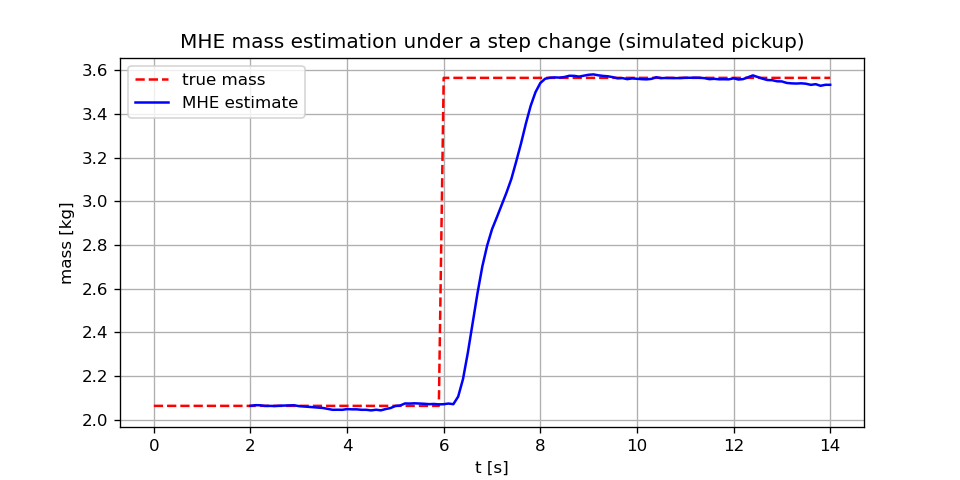
\includegraphics[width=0.92\textwidth]{Figures/mhe_mass_step.png}
\caption{Legacy fixed-weight MHE response to a simulated payload mass step.}
\label{fig:mhe-step}
\end{figure}

\section{No-Task-Mass Baseline Verification}

Revision \texttt{d1a8d30} added tests at three levels. First, cold-start
unit tests verify ground/thrust gating, convergence latching, publication
gating and the absence of an $m_b$ fallback. Second, an acados
observability test starts the same synthetic flight from the numerical
box midpoint and from the true value; its acceptance criteria are less
than \SI{5}{\percent} final error and less than \SI{0.05}{kg}
difference between final solutions. Third, a recorded
$T_{\mathrm{phys}}$ replay validates the signed step detector. Revision
\texttt{f2264b3} adds the bounded online-$\dJ$ path, regression tests for
its floor, cap, ratchet and gain-baseline semantics, and low-rate
\texttt{[mass-diag]} and \texttt{[dJ\_online]} records.

\begin{table}[ht]
\centering
\caption{Verification definition for the no-task-mass dissertation profile at revision \texttt{f2264b3}.}
\label{tab:noprior-verification}
\begin{tabularx}{\textwidth}{@{}p{0.28\textwidth} X@{}}
\toprule
\textbf{Property} & \textbf{Implemented check or recorded replay result} \\
\midrule
No mass answer in MHE & $Q_{0,m}=10^{-6}$, $m\in[0.2,5.0]$ kg and midpoint fallback; none contains $m_b$ or $m_p$ \\
Parcel prediction & $\hat m_p=(\hat m_t-m_b)^+$ is computed after optimisation; parcel truth is offline scoring only \\
Drop detection replay & three-sample half-windows, two-frame persistence; recorded drop detected after approximately \SI{0.30}{s} with a \SI{-2.37}{N} step \\
False-release protection & \SI{1.0}{N} schedules deweighting, but geometry release requires a negative step of at least \SI{2.0}{N}; the recorded figure-eight transition is therefore not allowed to release geometry \\
Drop regression & geometry is cleared but $\hat m_t$ is not reset; the acceptance script requires all three runs to return to $(2.064\pm0.03)\,\si{kg}$ and remain there \\
Online inertia update & \texttt{DJ\_TRACK\_MEST=1} maps the published $\hat m_p$ into $\dJ$ with a \SI{0.15}{kg} floor, \SI{0.6}{kg} cap and selectable ratchet; drop clears geometry and the ratchet, not the MHE mass state \\
Safety-information boundary & the MHE consumes no parcel envelope in coupled mode; the NMPC gain schedule still starts from a \SI{0.5}{kg} platform envelope, which must be reported and ablated \\
\bottomrule
\end{tabularx}
\end{table}

The replay also exposes an important limitation: a trajectory-mode change
can produce a real thrust step and may schedule MHE deweighting. The
higher signed release threshold prevents this event from declaring the
payload absent, but it does not make thrust-only change attribution
unique. This limitation is retained explicitly rather than hidden.

The same revision changes the unattended NMPC geometry-source default
from \texttt{truth} to \texttt{online}. The repository records an
eight-repetition comparison per arm: three of eight truth-source runs and
one of eight online-source runs failed. Fisher's exact test gives
$p=0.569$, while the five successful pairs satisfy the predeclared mass-
bias non-inferiority margin ($d=+0.025$ percentage points; upper
\SI{95}{\percent} confidence bound $+0.788<1.0$ percentage point). This
supports removal of joint truth from the default path, but it is not a
full validation result because the predeclared 16-of-16 success condition
was not met. The newly added MHE-envelope A/B script contains acceptance
logic but no frozen result set in the commit.

\draftnote{Run the acados cold-start test and the three-run drop-regression acceptance batch in the ROS~2/Linux environment, archive their complete console output and logs, and replace acceptance criteria in Table~\ref{tab:noprior-verification} with measured mean, spread and run identifiers.}

\section{Inherited Main-Branch SITL Results}

Table~\ref{tab:repo-results} records quantitative claims attached to the
preceding main revision \texttt{e003d339}. They motivate the event
schedule and numerical configuration, but they are not presented as
validation of the no-initial-mass baseline introduced in
\texttt{d1a8d30} and extended in \texttt{f2264b3}.

\begin{table}[ht]
\centering
\caption{Inherited SITL results reported for predecessor revision \texttt{e003d339}.}
\label{tab:repo-results}
\begin{tabularx}{\textwidth}{@{}X X@{}}
\toprule
\textbf{Comparison or metric} & \textbf{Reported result} \\
\midrule
Mass settling after a payload event & \SI{1.20}{s} fixed-weight versus \SI{0.30}{s} event-triggered (4.0$\times$ faster) \\
Residual-only trigger & settling time within \SI{0.02}{s} of the external-signal path \\
L1-adaptive NMPC comparison & comparable transient tracking; MHE--NMPC recovery reported as 15--35\% faster, with explicit mass/CoM parameters \\
NMPC computation at \SI{20}{Hz} & \SI{1.3}{ms} median and \SI{2.2}{ms} p99, equal to 4.4\% of the \SI{50}{ms} control period \\
Baseline matrix robustness & zero divergent runs out of 60 \\
Simulation-optimised MHE weights & no measurable gain over M0 in the paired factorial ablation \\
\bottomrule
\end{tabularx}
\end{table}

The negative weight-learning result is substantively useful. The objective was flat over a broad neighbourhood of the hand-designed rule: the performance improvement comes from identifying when the model changes and removing stale data, whereas the exact post-trigger weight magnitude is weakly determined. The trained schedule should therefore not be presented as a superior learned controller.

\draftnote{Audit Table~\ref{tab:repo-results} against the frozen logs and aggregation outputs before submission. Do not combine these predecessor results with the no-task-mass baseline results; report the latter as a new paired experiment matrix.}

\section{Final Evidence Layout}

To keep the final dissertation evidence-driven, the submission version should preserve the following order:
\begin{enumerate}
    \item one table of scenario parameters and repetition counts;
    \item estimator plots showing mass/CoM truth only for offline scoring;
    \item paired trajectory and error plots for fixed, adaptive and oracle controllers;
    \item constraint-margin and solve-time distributions;
    \item the payload mass--eccentricity success matrix;
    \item ablation results linked directly to the model entry points in Chapter~\ref{ch:model}.
\end{enumerate}

\section{Validity and Reproducibility}

The two scenario lines use independent world/configuration files so that direct inertial modification is not confused with detachable-body physics. Every run records the software revision, OCP dimensions, horizon, weights, payload geometry, event timestamps, random seed and solver statistics. Runs terminated by numerical failure remain in the mission-success denominator. Any manually excluded run must be identified with a predeclared hardware or logging fault. Revision \texttt{f2264b3} is the source-code anchor for the adopted algorithm, while \texttt{e003d339} is the anchor for the inherited figures in Table~\ref{tab:repo-results}. A defensible submission must freeze separate logs, manifests and aggregation outputs for the no-task-mass cold-start, pickup-prediction, online-inertia and drop-regression runs.

The main threats to validity are simulator-specific motor/thrust calibration, state estimates that are cleaner than real sensors, unmodelled contact oscillation, known attachment geometry and the remaining mass-valued safety floor/envelope. Hardware transfer must therefore begin with rotor-thrust calibration and conservative envelope tests rather than reusing the SITL limits unchanged. Claims about prior-free estimation must be kept separate from claims about a strictly mass-scale-free full controller.

\end{spacing}
\newpage
